\begin{figure}[htb!]
  \hspace{0.015\textwidth}
  \begin{subfigure}[b]{0.21\textwidth}
    \centering
    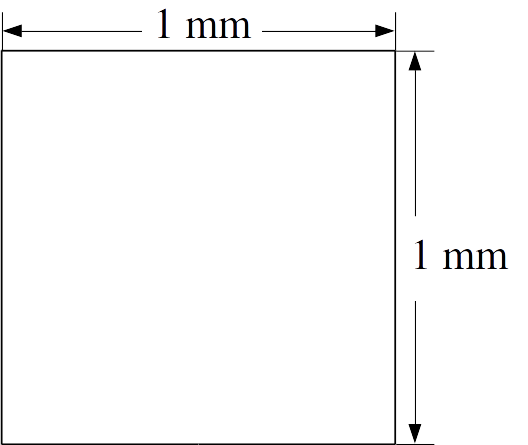
\includegraphics[width=\textwidth,scale=0.5]{Chapter4/figures/intact_plate_dimensions.png}
    \vspace{-0.03\textwidth}
    \caption{}
  \end{subfigure}
  \begin{subfigure}[b]{0.21\textwidth}
    \centering
    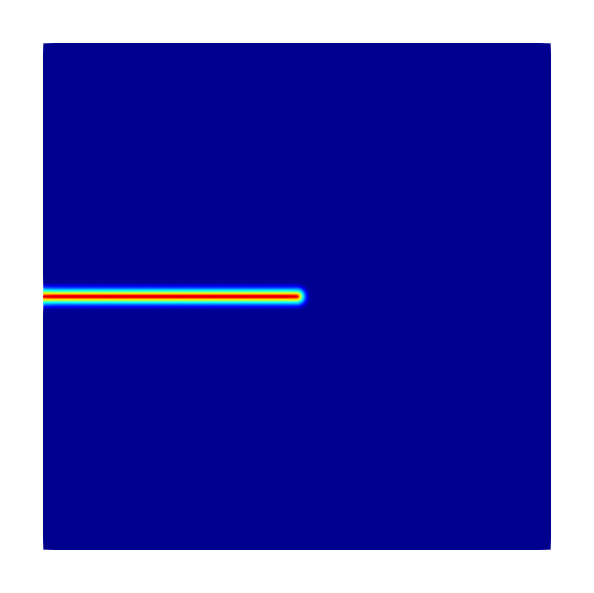
\includegraphics[width=\textwidth,scale=0.5]{Chapter4/figures/intact_plate_initial.png}
    \caption{}
    \label{fig: Chapter4/intact_plate_initial}
  \end{subfigure}
  \begin{subfigure}[b]{0.21\textwidth}
    \centering
    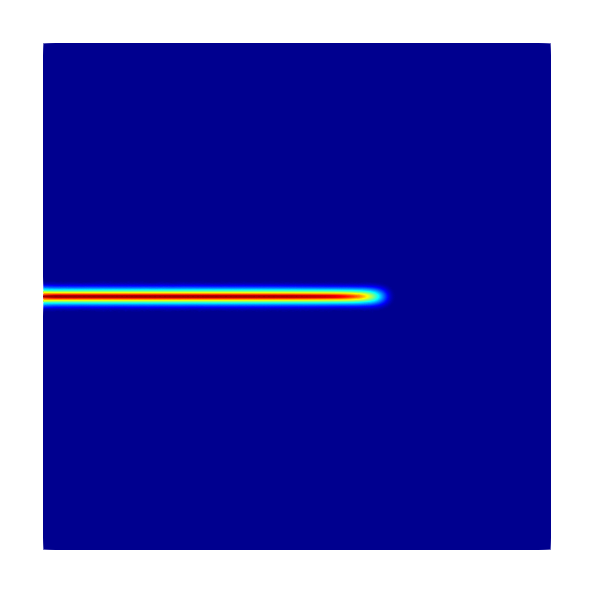
\includegraphics[width=\textwidth,scale=0.5]{Chapter4/figures/mode1_intact_plate_intermediate.png}
    \caption{}
  \end{subfigure}
  \begin{subfigure}[b]{0.21\textwidth}
    \centering
    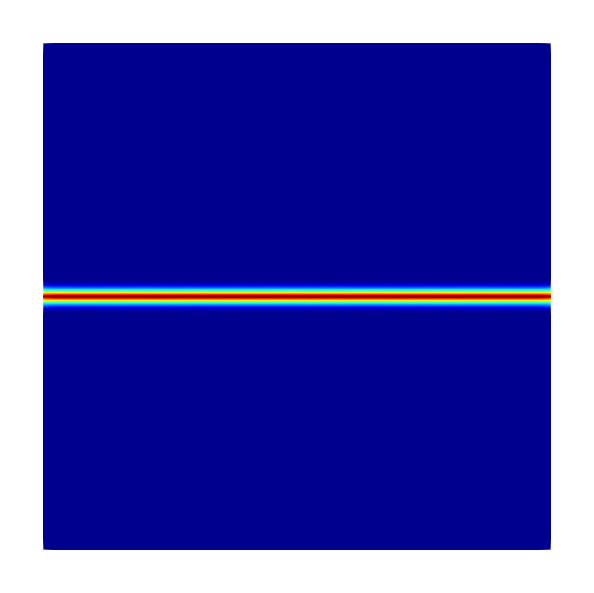
\includegraphics[width=\textwidth,scale=0.5]{Chapter4/figures/mode1_intact_plate_final.png}
    \caption{}
  \end{subfigure}
  \begin{subfigure}[b]{0.06\textwidth}
    \centering
    \caption*{d}
    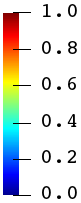
\includegraphics[width=\textwidth]{Chapter4/figures/jet_vertical.png}
    \vspace{0.15in}
  \end{subfigure}
  \caption{ Edge-notched specimen loaded in tension  with initial crack represented by a damage field.  (a) Dimensions of the intact plate. The  Damage $d$ at (b) $u_y = \SI{0}{\milli\meter}$ (c) $u_y = \SI{0.0048}{\milli\meter}$ (d) $u_y = \SI{0.006}{\milli\meter}$. }
  \label{fig: Chapter4/mode1_intact_plate}
\end{figure}
